\documentclass[conference]{IEEEtran}
\IEEEoverridecommandlockouts
% The preceding line is only needed to identify funding in the first footnote. If that is unneeded, please comment it out.
\usepackage{cite}
\usepackage{amsmath,amssymb,amsfonts}
\usepackage{algorithmic}
\usepackage{graphicx}
\usepackage{textcomp}
\usepackage{xcolor}
\usepackage{longtable}
\usepackage{stmaryrd}
\usepackage[numbers]{natbib}

\pagestyle{plain}
\newcommand{\paraheading}[1]{{\color{blue}\textit{#1}}}
\usepackage{hyperref}

\def\BibTeX{{\rm B\kern-.05em{\sc i\kern-.025em b}\kern-.08em
    T\kern-.1667em\lower.7ex\hbox{E}\kern-.125emX}}
\begin{document}


\title{Scheduling time-triggered tasks in multicore real-time systems: a machine learning approach\\
%{\footnotesize \textsuperscript{*}Note: Sub-titles are not captured in Xplore and
%should not be used}
%\thanks{Identify applicable funding agency here. If none, delete this.}
}

\author{\IEEEauthorblockN{Félicien Fiscus-Gay}
\IEEEauthorblockA{\textit{Computer Science} \\
\textit{Auckland University of Technology}\\
Auckland, New Zealand \\
felicien.fgay@gmail.com}
}

\maketitle
\thispagestyle{plain}

\begin{abstract}
\textit{Background}: Previous research and/or rationale for performing the study.

\textit{Aims}: Hypotheses/propositions to be tested, or goal of the study.

\textit{Method}: Description of the type of study, treatments, number and nature of
experimental units (people, teams, algorithms, programs, tasks etc.), experimental
design, outcome being measured.



\textit{Results}: Treatment outcome values, level of significance.


\textit{Conclusions}: Limitations of the study, implications of the results, and further work
\end{abstract}

\begin{IEEEkeywords}
real-time system, scheduling, time-triggered tasks, DAG, multicore
\end{IEEEkeywords}


\section{Introduction}
\label{sec:intro}

Real-time systems are utilized in various domains such as air traffic 
control, public transportation, and automated vehicles. Unlike non-real-time systems, 
tasks in real-time systems must be both functionally correct and meet strict 
(or flexible) execution time constraints, known as deadlines. Failure 
to meet these deadlines can lead to severe consequences. The critical 
nature of these systems necessitates designing the system 
architecture with a focus on time and incorporating fault tolerance 
to ensure high reliability.

One example of such architecture is the time-triggered 
architecture (TTA)\cite{kopetz2003tta}\cite{kopetz1998timetriggered}, which offers a fault-tolerant communication protocol and a precise timing system to synchronize different electronic control units. Developing and running tasks on these architectures require in-depth knowledge of the system and its architecture, which complicates code reusability and scalability when adding hardware resources or upgrading to a larger system.

To address these issues, the Automotive Open System Architecture 
(AUTOSAR\footnote{\url{https://www.autosar.org/}}) was developed. 
AUTOSAR introduces layers of abstraction between hardware, firmware, 
and software, enhancing software reusability and hardware 
scalability across different systems while maintaining safety and 
security standards. It is now the most widely used architecture among car 
manufacturers, with notable core partners including BMW, Ford, and Toyota.

Scalability, in particular, plays a crucial role in modern 
real-time systems. Increasingly, real-time systems such as 
autonomous cars or computer vision systems are enhancing their 
computational resources by transitioning to multiprocessor systems. 
This shift from uniprocessor to multiprocessor systems addresses 
the growing complexity and computational demands of tasks executed 
on these systems, aiming to reduce both the execution time of these 
tasks and the required resources\cite{maiza2019survey}.

Hence, an increasing number of real-time systems are 
utilizing multi-core hardware to parallelize their tasks 
and convert sequential programs into parallelized ones using 
frameworks such as OpenMP
\footnote{OpenMP (2011) OpenMP Application Program Interface v3.1. 
\url{http://www.openmp.org/mp-documents/OpenMP3.1.pdf}}. 
Unfortunately, in most real-life scenarios, the number of available 
processors/cores is fewer than the number of tasks/subtasks that 
can be executed in parallel (i.e., independent tasks). This means 
that not all independent tasks can be executed simultaneously on 
the system, raising the question: which task should be executed first?

This question is particularly important in a real-time context 
because having the wrong execution order, or schedule, could lead 
to, at best, a slow system, and at worst, deadline misses, which 
can have fatal repercussions. In the case of a self-driving car 
system, for instance, a slight delay of 500 ms in detecting a pedestrian 
crossing the road can, in some cases, be enough to drive over 
the pedestrian or cause a car accident. Note that the resources of 
real-time systems are scarce and limited, which is why using as 
little processing power as possible while ensuring that tasks meet 
their deadlines is of crucial importance.

The extreme case of this scheduling problem arises when only one 
processor is available to execute tasks. This is known as task 
scheduling on a uniprocessor, and \cite{liu1973scheduling} 
provided two major priority policies: Rate Monotonic (RM) and 
Earliest Deadline First (EDF) for scheduling periodic tasks. 
However, when considering multiple processors, the scheduling 
problem becomes much more complex, and different task models must 
be considered.

A prevalent task model is the time-triggered task model, 
which specifies tasks that execute periodically and is well-suited 
for time-triggered systems. Another type of task is the Logical 
Execution Time (LET) task. The LET paradigm is based on the 
time-triggered paradigm and was originally introduced by the 
Giotto real-time programming language\cite{henzinger2003giotto} and 
later refined by \cite{henzinger2009distributed} into the 
Hierarchical Timing Language (HTL). The main principle behind the 
LET paradigm is that each task's inputs and outputs are read and 
written in zero time, i.e., constant time.

The benefits of using LET are twofold. Firstly, the zero-time 
communication semantics greatly improve the predictability of the 
overall system and make I/O operations (i.e., memory access) on 
shared resources deterministic, which is crucial in real-time 
systems due to the highly negative impact that memory access 
contentions can have on the system\cite{nagalakshmi2016impact}. 
Secondly, using LET in programming also provides a layer of 
abstraction that facilitates the direct translation from modeling 
to implementation, thus ensuring the implementation of timing 
requirements, enhancing code maintenance, and producing a less 
error-prone code base\cite{kirsch2012logical}.

One drawback of LET is its implementation overhead, which increases 
the execution times of tasks due to the zero-time communication 
semantics\cite{biondi2018LETruntimeoverhead}. Despite this drawback, 
the advantages of LET make it attractive for real-time systems\cite{gemlau2021systemLET}, 
which is why the focus here will be on time-triggered and LET 
task scheduling on multi-core systems. Given that the problem of 
scheduling independent tasks is NP-hard\footnote{If a problem is 
NP-hard, it means that it is very unlikely to find a solution in 
polynomial time complexity, i.e., solutions are not scalable}\cite{du1989schedNPhard}, 
no scalable optimal algorithm exists. Therefore, heuristics are 
used to partially solve the problem.

Consequently, machine learning will be considered here as it can 
better approximate the unattainable perfect solution while being 
scalable in terms of computing time after the training phase. In 
other words, the research questions are:

\begin{itemize}
    \item [RQ1] What is the current state-of-the-Art in scheduling event-chains of tasks ?
            \begin{itemize}
                \item [RQ1.1] What is the current state-of-the-Art for DAG task scheduling with precedence constraints ?
                \item [RQ1.2] How has LET been used in scheduling event-chains ?
                \item [RQ1.3] What machine learning  techniques are used for DAG task scheduling ?
            \end{itemize}
    \item [RQ2]  Can machine learning be a better solution to schedule event-chains of tasks ?
            \begin{itemize}
                \item [RQ2.1] Can a machine learning solution compare to state-of-the art heuristics for scheduling Directed Acyclic Graph tasks ?
                \item [RQ2.2] Can a machine learning solution compare to ILP solutions while being more scalable ?
            \end{itemize}    
\end{itemize}

To achieve this, the background section will introduce various 
technical terms, concepts, and fundamental algorithms. 
Following this, a systematic literature review will be conducted to address R1, 
and finally, the artifact and experimental design, results, and conclusion will 
be presented to answer R2.



\paraheading{The solution we propose has the following features..}

\paraheading{The primary contributions of this paper are:}


\section{Background}
\label{sec:bg}

Task scheduling introduces several fundamental concepts.

\subsection{Periodic task and schedule}
~

Firstly, a periodic task $\tau_i(C_i, D_i, T_i)$ is characterized 
by its worst-case execution time (wcet) $C_i$, its deadline $D_i$, and 
its period $T_i$. This definition can be expanded by including an 
initial offset, which corresponds to the time of the task's first 
execution, and an activation offset, which is the time delay between 
the task being ready to execute (i.e., its execution period has begun) 
and the task actually starting to run. Secondly, a schedule $S$ is a 
function that assigns a boolean value for each task $\tau$ and each 
time tick $t$, indicating whether the task $\tau$ is running at 
time $t$. Therefore, a scheduling algorithm is the method that, 
given a set of tasks, produces a schedule $S$ for the task set.

This task model and schedule definition are widely adopted in the literature (see section \ref{sec:literature}) 
and are the building blocks of all scheduling algorithms.
The periodic task model, in particular, is used to define more complex
tasks such as DAG tasks (see below) that will be used as input in the 
machine learning model (see section \ref{sec:methodology}).

\subsection{DAG task}
~

A Directed Acyclic Graph (DAG) task 
is a task that models the multiple subtasks of an chain of tasks
that have a precedence constraints.
For example, when considering the task $\tau_1$ that makes an 
aircraft keep its altitude, you usually have a number of subtasks
to handle this task, namely : reading from the altitude sensor ($\tau_{11}$),
reading for the speed sensor ($\tau_{12}$), computing the new speed for the aircraft
to keep its altitude ($\tau_13$), computing the amount of thrust needed to achieve
this new speed ($\tau_14$), and finally actuating the aircraft's jet engine ($\tau_15$).
In this example, the DAG for $\tau_1$ can be seen in Figure \ref{fig:dag_example}.

\begin{figure}
    \centering
    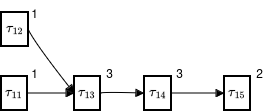
\includegraphics[width=0.5\linewidth]{images/example_dag.png}
    \caption{DAG task $\tau_1$. The nodes are the subtasks,
    the edges of the graph represent the precedence constraints between each subtasks and the worst-case execution time (wcet) of each subtask written as an exponent.}
    \label{fig:dag_example}
\end{figure}

A DAG task $\tau_i$ also has a period $T_i$ and a wcet $C_i$ which 
is the sum of its subtasks wcets, and a deadline $D_i$.
For instance, according to Figure \ref{fig:dag_example},
the wcet for $\tau_1$ is 10 time units.
You can also see how, for $\tau_1$, 
the subtasks $\tau_{12}$ and $\tau_{11}$ can be parrallelized (i.e., 
executed in parallel) but the subtask $\tau_{13}$ needs to wait 
for both $\tau_{11}$ and $\tau_{12}$ to finish their execution 
before it can start running.
\\

This concept will be the task model used in to conduct 
part of the systematic literature review (see Section \ref{sec:literature})
and it also will be the task model used for designing 
the machine learning model (see Section \ref{sec:methodology}).


\subsection{Utilization factor}

The utilization factor represents the percentage of processing 
time that a taskset $(\tau_1, \cdots, \tau_n)$ will utilize. 
Formally, it is defined as
\begin{align}
U = \sum_{k=1}^{n} \frac{C_k}{T_k}
\end{align}
where $U$ is the utilization factor. This concept is significant 
because, when evaluating a scheduling algorithm $S$, we desire 
$S$ to effectively schedule tasksets that maximize the utilization 
factor $U$. Consequently, the higher the utilization factor bound 
for $S$, the more efficient the scheduling algorithm. Additionally, 
this concept is valuable in real-time systems where processing 
resources are often limited and expensive, making it crucial to 
maximize their usage.

This concept is also used either as a measurement
when comparing two scheduling algorithms (see Section \ref{sec:literature}),
or used as a parameter to generate tasksets or DAG tasks with 
a fixed utilization (see Section \ref{sec:methodology}).

\subsection{Makespan}

The makespan or end-to-end response time of a 
DAG task is the amount of time it takes for all the subtasks
in the DAG task to finish executing when given a schedule.
For instance, for the task $\tau_1$ shown in Figure \ref{fig:dag_example},
the makespan of $\tau_1$ for the schedule shown in Figure \ref{fig:schedule_example}
is 9.
Notice that in Figure \ref{fig:schedule_example},
if the subtasks $\tau_{11}$ and $\tau_{12}$ were executed 
sequentially instead of in parrallel, the makespan would be 
one time unit longer, in this case 10 instead of 9.

\begin{figure}
    \centering
    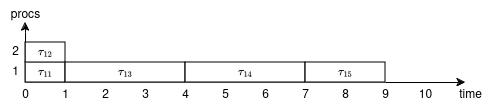
\includegraphics[width=0.5\linewidth]{images/schedule_example.png}
    \caption{Example of schedule for $\tau_1$. The y axis represents the number
    of processors that are not idle. For the first two subtasks there are two processors
    active and for the rest there is only one active processor.}
    \label{fig:schedule_example}
\end{figure}

This is a key measurement when dealing with DAG tasks (see Section \ref{sec:literature})
and it will be the main efficacy criteria when comparing 
the machine learning model with state-of-the-art heuristics and ILP
(see Section \ref{sec:methodology}).

\subsection{Acceptance ratio}

When dealing with several independent DAG tasks
or tasksets, 
the acceptance ratio is often used to measure the 
performance of a scheduling algorithm (see Section \ref{sec:literature}).
It consists of looking at a number of generated tasksets (or DAG tasks)
and calculating the amount of schedulable (i.e., 
the schedule produced doesn't lead to a deadline miss) tasksets compared to 
the total amount of taskets.
The resulting percentage is the acceptance ratio 
and the closer it gets to 100\% for a scheduling algorithm, the better the scheduling algorithm.

This concept is also used as a measurement, to assert the efficiency
of scheduling algorithms when considering independent tasks (see Section \ref{sec:literature}).

%\cite{tiryaki2006sunit} is really good with MAS but really bad with something else.
\subsection{Optimality}

A scheduling algorithm $S$ is said to be optimal 
when the following condition is true:
for every taskset $\Omega$, if there exists 
a scheduling algorithm $S'$ so that $\Omega$ is feasible by $S'$,
then $\Omega$ is also feasible by $S$.
Where {\it{feasible}}, 
means that, using the schedule generated by $S$,
all the tasks in the taskset will finish executing before their deadlines.

This concept is used in the literature, mainly for independent tasks scheduling
(see Section \ref{sec:literature}).

\subsection{Approximation ratio}

The approximation ratio is the comparison between 
the average number of processors required by a scheduling algorithm 
to make a random taskset feasible and the average number of 
processors needed by the theoretically optimal scheduling algorithm 
for the same taskset.

It is a way of measuring scheduling algorithms,
especially when considering independent tasks (see Section \ref{sec:literature}).
\\


While the acceptance and approximation ratio are used 
to measure the performance of scheduling alrogithms for independent tasks,
the makespan is only used for DAG tasks and tasksets representing chain of events.

\subsection{RM and EDF scheduling}
~

When designing a scheduling algorithm, the key decision involves 
determining which task should execute first when two or more 
independent tasks are ready to execute. This requires assigning each 
task a priority. \cite{liu1973scheduling} introduced two 
heuristics for this purpose: Rate Monotonic (RM) and Earliest 
Deadline First (EDF).

The RM algorithm is a fixed-priority scheduling algorithm, 
meaning that the priority of each task is known before execution 
begins. RM assigns the highest priority to tasks with the minimum 
execution rate, i.e., $\frac{C_k}{T_k}$, and is considered optimal 
for assigning fixed priorities to tasks. In contrast, EDF assigns 
priorities dynamically by selecting tasks based on which one has 
the earliest absolute deadline.

Figure \ref{fig:edf_rm_examples} illustrates the difference 
between the two algorithms by scheduling the same two tasks, 
$\tau_1$ and $\tau_2$. $\tau_1$ has a worst-case execution time of 0.5 time units 
and a period of 2 time units, while $\tau_2$ has a worst-case execution 
time of 2 time units and a period of 3 time units. These are 
examples of implicit deadline tasks, where the relative deadline 
equals the end of their execution period. 

\begin{figure}
    \centering
    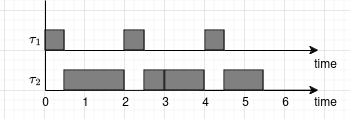
\includegraphics[width=\linewidth, height=100px]{images/schedule_rm.png}
    a)
    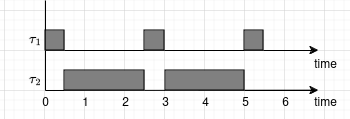
\includegraphics[width=\linewidth, height=100px]{images/schedule_edf.png}
    b)
    \caption{Schedules of $\tau_1$ and $\tau_2$ using Rate Monotonic (a)
    and Earliest Deadline First (b) heuristics.}
    \label{fig:edf_rm_examples}
\end{figure}

Although EDF calculates each priority at runtime, it is optimal 
for uniprocessor scheduling and has a theoretical utilization bound 
of 1, which is the maximum possible for a feasible taskset on a 
single processor. RM, on the other hand, has a much lower 
utilization bound than EDF. While one might argue that RM introduces 
less runtime overhead and is therefore more practical, it has been 
shown that RM leads to more task preemptions (interrupting the 
execution of a task, as seen at times 2 and 4 for task $\tau_2$ in 
Figure \ref{fig:edf_rm_examples}.a). This, combined with its lower 
utilization bound and non-optimality, makes EDF clearly superior to 
RM\cite{buttazzo2005RMvsEDF}.

Although \cite{liu1973scheduling}'s work focused on uniprocessor 
systems, the proposed algorithms have also been applied to 
multi-processor scheduling.

\section{Related Works}
\label{sec:literature}

\subsection{Systematic Literature Review process}

\paraheading{\textbf{Scoping}}

This SLR aims at tackling RQ1. More precisely, the following research questions will be answered:

\begin{itemize}
    \item [RQ1.1] What is the current state-of-the-Art for DAG task scheduling with precedence constraints ?
    \item [RQ1.2] How has LET been used in scheduling event-chains ?
    \item [RQ1.3] What machine learning techniques have been used for scheduling tasks on real-time systems ?
\end{itemize}
It will also be shown how the literature doesn't provide 
a complete answer to RQ2, hence the contributions of this paper.\\

From these research questions, several concepts have been isolated,
namely, time-triggered tasks, the nature of the system (real-time multicore system),
the scheduling of tasks, DAG tasks, and machine learning.
The recording of the search results were done using the BibTeX LateX plugin
combine with the google scholar "cite" feature.

Searching was conducted using the IEEE and ACM databases.
According to the concepts identified above, 
the keyword chain used for searching was 
"("real-time" OR "real time") AND 
"system" AND ("time-triggered" OR "time triggered" OR "DAG" OR "Directed Acyclic Graph" OR "LET" OR "Logical Execution Time" OR "event chain" OR "event-chain") 
AND "task" 
AND ("scheduling" OR "scheduler" OR "schedule") 
AND ("multi-processors" OR "multi-cores" OR "multi processors" OR 
"multi cores" OR "multi-processor" OR "multi processor" OR 
"multi-core" OR "multi core")".

The search produced 3,549 results on the IEEE database

exclusion : past 5 years : IEEE --> down to 1,171 
            heterogeneous not in title + abstract : IEEE --> down to 999
            mixed critical* not in title + abstract : IEEE --> down to 952
            scheduling or scheduler or schedule in title but not "energy" :  IEEE --> down to 155 and 149 when just considering conference and journal papers (not early access)
            
            removing those not about real-time system,
            not about proposing a scheduling algorithm,
            not about DAG nor LET tasks or event-chains : IEEE --> down to 21

\paragraph{}

\subsection{Findings of the Literature Review}

\paraheading{The works reviewed were compared on the following metrics.} 
\begin{itemize}
    \item \textbf{Utilization Bound}: useful to see which algorithm is more efficient at using the available resources.
    \item \textbf{Acceptance Ratio}: it shows how optimal (see Section \ref{sec:bg}) a scheduling algorithm is.
    \item \textbf{Makespan}: for DAG task scheduling, widely used in the literature.
    \item \textbf{Runtime Overhead}: some scheduling algorithms can show promising results theoretically but are practically very slow because 
    of their complexity adding runtime overhead on the scheduler, this metric will not be a number but rather an amount such as minimal, practical, non-practical.
\end{itemize}
Every metric used here have also been chosen for their prevalence in the literature.

A comparison of the works was carried out and the overall results are illustrated in Table~\ref{tab:slrtable}.
 

\begin{table}
    \centering
    \begin{tabular}[]{|l|p{0.20\linewidth}|p{0.20\linewidth}|p{0.20\linewidth}|}
        \hline
        \textbf{Reference} & \textbf{Scheduling technique} & \textbf{Task type} & \textbf{Scope (intra/inter/both)}\\
        \hline
        \cite{guan2021DAGfluid} & fluid & implicit deadline & inter\\
        \hline
        \cite{He2019DagIntra} & priority-list & constrained deadline & intra \\
        \hline
        \cite{Kobayashi2023FedBundledDagsched} & federated and bundled-based & constrained deadline & inter\\
        \hline
        \cite{Xiao2019}  & clustering & constrained deadline & intra\\ 
        \hline
        \cite{Igarashi2020HeuristicContentionFree}  & priority-list & LET constrained deadline & both \\
        \hline
        \cite{jiangUtilTensityBound}  & federated and GEDF and PEDF & implicit deadline & inter\\
        \hline
        \cite{JiangDecompoSchedParallelTask} & Decomposition-based & implicit deadline & inter \\
        \hline
        \cite{He2023DegreeOfParallelism} & federated-based & constrained deadlines & inter \\
        \hline
        \cite{Shi2024DagExecGroups}  & partitioned / clustering & constrained deadlines & intra\\
        \hline
        \cite{Guan2023FederatedNew}  & federated & arbitrary deadline & inter\\
        \hline
        \cite{Zhao2024GATDRLmodel} & DRL & constrained deadline & intra\\
        \hline
        \cite{Xu2023DRLtaskSched} & DRL & non-DAG implicit deadline & inter\\
        \hline
        \cite{Zhao2022DAGsched} & priority-list and federated & constrained deadline & both \\
        \hline
        \cite{Lee2021GlobalDagSchedDRL} & DRL & constrained deadline & intra\\
        \hline
        \cite{Jiang2023SchedVirtualProcs} & federated-based & constrained deadline & inter\\
        \hline
        \cite{GuanFluidDag2022} & fluid & constrained/arbitrary deadline & inter\\
        \hline
        \cite{GuanFRTDS2020RL} & DRL & constrained deadline & intra \\
        \hline
        \cite{JiangVirtuallyFederatedSched2021} & federated-based & constrained deadline & inter\\
        \hline
        \cite{Pazzaglia2021DMALETtransfer} & Mixed ILP & LET, constrained deadline & inter\\
        \hline
        \textbf{Total: 19} & \textbf{DRL: 4, Federated: 7, Fluid: 2, ILP: 1, Priority-List(intra): 3, Clustering: 2, Decomposition: 1}
        & \textbf{implicit: 4, constrained: 13, arbitrary: 2} & \textbf{inter: 11, intra: 6, both: 2} \\
        \hline
    \end{tabular}
    \caption{SLR summary table}
    \label{tab:slt_sum_table}
\end{table}


\subsubsection{DAG tasks}
~

Scheduling DAG tasks involves two steps: first, 
computing the intra-task schedule, and second, computing 
the inter-task schedule. For the inter-task schedule, various 
approaches can be employed.

\cite{WangGEDFDag2019}, for instance, improve the worst-case 
makespan of GEDF under federated scheduling of multiple DAG tasks 
with arbitrary deadlines. The federated scheduling approach, 
similar to the partitioning approach, involves assigning clusters 
of processors to DAG tasks with the highest utilization, leaving 
the remainder for low-utilization tasks. This allows for 
intra-task parallelization instead of merely sequentializing 
the DAG task. Consequently, the paper also improves the acceptance 
ratio for single DAG task scheduling by providing a better 
schedulability test compared to previously used 
schedulability tests for GEDF.

Another method is the decomposition approach, which involves 
decomposing the DAG task into several independent sequential tasks. 
These tasks are then executed in parallel segments, with their 
release times and deadlines aligned to match the dependency constraints 
between the sequential tasks\cite{CaoStretchingDAGs2020}. The paper 
\cite{CaoStretchingDAGs2020} introduces a state-of-the-art 
stretching method for DAG task decomposition and employs the GEDF 
dynamic priority assignment algorithm to demonstrate improvements 
in the acceptance ratio over the previous state-of-the-art 
decomposition algorithm.

\cite{SchmidResponseDAGThreadpools2021} explores a thread pool 
approach for parallelizing DAG tasks. Instead of assigning 
processors to DAG tasks, thread workers from a thread pool are 
assigned, and the number of thread workers each DAG can use is 
limited. Their algorithm, combined with a global fixed-point 
priority scheduling algorithm such as Rate Monotonic, is compared 
to other approaches, including the global approach and the 
semi-federated approach.

The global approach does not assign processors to DAG tasks but 
allows the tasks to utilize multiple processors dynamically. 
The semi-federated approach, similar to the federated approach, 
places as many heavy tasks (tasks with high utilization) in processor 
clusters as possible, while the remaining tasks, along with the 
light tasks, are allocated to the rest of the available processors.

It is found that the latest approach generally outperforms 
the method used in \cite{SchmidResponseDAGThreadpools2021}, although the 
thread pools approach still has a better acceptance ratio compared 
to the global approach.

The previously cited articles focus on the execution of multiple 
DAGs on a multi-processor system, utilizing existing priority 
scheduling algorithms such as GEDF or Global RM to evaluate their 
contributions. \cite{he2019intra} considers recurrent DAG tasks 
and their inner graph structure to develop a priority assignment 
algorithm that minimizes the makespan of the DAG task. This 
algorithm is then extended to multi-DAG scheduling using a global 
scheduling approach such as G-EDF or G-RM. This dynamic scheduling 
approach performs best with G-RM in terms of acceptance ratio.

The results in terms of acceptance ratio are superior to those in 
\cite{SchmidResponseDAGThreadpools2021}, though in some cases they 
are surpassed by \cite{CaoStretchingDAGs2020}. However, a 
drawback of \cite{CaoStretchingDAGs2020} is that this type of task 
decomposition incurs significant runtime overhead, which diminishes 
task performance in real-life scenarios.

While \cite{he2019intra} and \cite{CaoStretchingDAGs2020} allow 
for task preemption, which especially in the case of 
\cite{CaoStretchingDAGs2020} adds runtime overhead, 
\cite{zhao2020dag} leverages the parallelism and dependency 
properties of DAG tasks, along with a 'critical path first' 
execution strategy, to develop a state-of-the-art non-preemptive 
and priority-based scheduling algorithm that completely outperforms 
\cite{he2019intra} in terms of makespan. Their results are utilized 
by \cite{lee2021DAGDeeplearning} to compare with a deep 
learning-based priority assignment algorithm for DAGs, which 
improves the makespan of DAG task execution by 2$\sim$3\%.

\cite{zhao2022dag} extends their concurrent provider and consumer 
(CPC) model \cite{zhao2020dag} to multi-DAG scheduling by 
minimizing inter-task DAG interference to zero and devising a 
processor-assigning scheduling algorithm where the priority of 
different DAG tasks is computed using the deadline-monotonic 
algorithm. Under non-preemptive scheduling, the proposed method 
significantly outperforms the method used in \cite{he2019intra} in 
terms of acceptance ratio, by up to 60\%.

For multi-DAG scheduling, \cite{GuanDAGfluid2021} employed the 
fluid scheduling strategy to manage DAG tasks with implicit 
deadlines. This fluid scheduling approach, also used in PFair and 
LLREF scheduling algorithms \cite{baruah1993PFair}\cite{cho2006LLREF}, 
ensures that at every point in time, each task has utilized the 
amount of execution time dictated by its respective utilization 
factor, thereby approximating the perfect fluid execution of the 
task. The advantage of this approach is its exceptionally high 
acceptance ratio, outperforming other methods such as 
\cite{WangGEDFDag2019}, \cite{he2019intra}, and \cite{CaoStretchingDAGs2020}. 
However, it suffers from high runtime overhead, complicating 
practical implementation.
\newline

A more mathematical approach to the scheduling of DAGs is to model 
the scheduling problem as an Integer Linear Programming (ILP) 
optimization problem. In this model, precedence, deadline, and 
processor assignment constraints are represented mathematically, 
with the objective of minimizing the makespan. This method is 
utilized by \cite{ChangMinWRCTBoundILP2022} and compared to 
state-of-the-art priority assignment algorithms (\cite{he2019intra} 
and \cite{zhao2020dag}). The ILP method demonstrates a significant 
improvement in makespan, which is expected due to the optimality of 
the ILP approach. However, the drawback of this method is that as 
the number of tasks and subtasks increases, the number of 
constraints grows, causing the computation time to increase 
exponentially, rendering the method non-scalable.

Most studies do not consider the communication time between tasks, 
which can be significant in real-life systems. 
\cite{ChenDAGorder2023} addresses this by scheduling DAG tasks on a 
Network on Chip (NoC) system. The resulting schedule, DAG-Order, 
is non-preemptive and is based on ordering the tasks according to 
their communication delays and computation workloads.

Memory access contention, which occurs when two or more tasks 
attempt to access a shared memory location simultaneously, can 
also be crucial in real-life scenarios. Therefore, scheduling 
algorithms for implementations of the LET paradigm have been 
proposed to reduce or even eliminate contention problems with LET 
DAG tasks \cite{Yano2021ContentionFree}\cite{Igarashi2020HeuristicContFree}.
\newline


The machine learning community has also explored DAG scheduling. 
For instance, \cite{yano2021work} utilized reinforcement 
learning (RL), specifically Q-learning, to statically prioritize 
sub-tasks within DAG tasks and applied an 
earliest-start-first (EST) heuristic value to dispatch each 
sub-task to different processors. Similar to \cite{ChenDAGorder2023}, 
\cite{yano2021work} accounted for communication delays and the 
workload of subtasks when assigning priorities.

Another application of RL is demonstrated by 
\cite{lee2021DAGDeeplearning}, who designed a deep learning model 
based on RL that uses the spatial features of each DAG task as well 
as their temporal features, i.e., precedence constraints. They 
achieved this by combining a graph convolution network 
(for spatial information) with a sequential encoder 
(for temporal information), ultimately producing a prioritized list 
of the DAG's subtasks. This list can then be used to compute 
the makespan and optimize it via RL. The results in 
\cite{lee2021DAGDeeplearning} were compared with state-of-the-art (SOTA) 
algorithms \cite{he2019intra}\cite{zhao2020dag}, with the deep 
reinforcement learning method surpassing the SOTA by up to 3\% 
in terms of makespan.

\begin{table}[htb]
    \centering
    \begin{tabular}[]{|l|p{0.20\linewidth}|p{0.35\linewidth}|}
        \hline
        $\mathbf{References}$ & $\mathbf{Category}$ & $\mathbf{Method}$ \\
        \hline
        \cite{CaoStretchingDAGs2020}\cite{GuanDAGfluid2021} & Decomposition & task segmentation and processor
        exclusivity for critical path\cite{CaoStretchingDAGs2020}, and fluid scheduling\cite{GuanDAGfluid2021}\\
        \hline
        \cite{WangGEDFDag2019}\cite{SchmidResponseDAGThreadpools2021}\cite{zhao2022dag}\cite{ChenDAGorder2023} & Partitioned/ Federated & Federated scheduling for inter-DAG scheduling and GEDF for intra-DAG\cite{WangGEDFDag2019}, 
        global preemptive fixed-priority scheduling using assigned thread-workers based on DAG workload\cite{SchmidResponseDAGThreadpools2021},
        workload and no inter-task interference based processor assignment with CPC model for intra-task priority assignment\cite{zhao2022dag},
        federated and order-based intra-task priority assignment based on workload and communication delays\cite{ChenDAGorder2023}\\
        \hline
        \cite{he2019intra} & Global & G-RM and G-EDF for inter-task and priority assignment by maximizing intra-task parralelism for intra-task scheduling\\
        \hline
        \cite{ChangMinWRCTBoundILP2022} & ILP & Only interested in intra-task interference, uses Integer Linear Programming to minimize the makespan\\
        \hline
        \cite{yano2021work}\cite{lee2021DAGDeeplearning} & Reinforcement Learning & Q-learning with partitioning at the intra-task level using EST heuristic\cite{yano2021work},
        GCN\footnotemark and sequential encoding priority assignment for a single DAG task and then use a work-conserving GFPS\footnotemark to assign tasks to processors\cite{lee2021DAGDeeplearning}\\
        \hline
        \cite{Igarashi2020HeuristicContFree}\cite{Yano2021ContentionFree} & mixed global / partitioned & blocks access from main tasks to certain cores to avoid contention
        by interpreting I/O operations as tasks with precedence constraints and parallelizing the main tasks\\
        \hline
    \end{tabular}
    \caption{Summary table for DAG task scheduling.}
    \label{tab:sum_table}
\end{table}


%\begin{table}[htb]
%\caption{Systematic Literature Review Results (Generate tables from \url{www.tablesgenerator.com})}
%\label{tab:slrtable}
%\begin{tabular}{|l|l|l|l|l|}
%\hline
%             & Metric 1 & Metric 2 & Metric 3 & Metric 4 \\ \hline
%{[}Work 1{]} &          &          &          &          \\ \hline
%{[}Work 2{]} &          &          &          &          \\ \hline
%{[}Work 3{]} &          &          &          &          \\ \hline
%{[}Work 4{]} &          &          &          &          \\ \hline
%\end{tabular}
%\end{table}

As you can see, although dynamic priority algorithms outperform 
fixed-priority ones, the simplicity of implementation and low runtime 
overhead of fixed-priority algorithms make them attractive to the 
industry. This is especially true for the DAG task model, where 
there has been significant focus on fixed-priority scheduling. While 
some have attempted to produce an 'optimal' schedule using 
ILP\cite{wei2011reliabilityILP}\cite{yip2014relaxing}\cite{ChangMinWRCTBoundILP2022}, 
the primary issue with this method is its lack of scalability.

Regarding task migrations, the NP-hard nature of the 
bin-packing problem suggests that allowing tasks or subtasks to migrate 
between processors can improve utilization performance.


Also, only 3 articles used machine learning to tackle the task scheduling problem,
from which two are from the same author.
Furthermore, those articles only compare their results to 
heuristic-based methods and not ILP methods.
If we focus on DAG tasks, then only 2 papers are left,
one focusing on communication between the cores and
applying the model on a specific architecture\cite{yano2021work},
and one more theoretical\cite{lee2021DAGDeeplearning}, comparing their model to SOTA 
\cite{zhao2020dag} and \cite{he2019intra}. The latter suffers 
from closed sourcing as their model is not open source
which prohibits the research community to improve on their work. 

Hence, there not only is a need to compare one such machine learning technique 
to the non-scalable but leading to the mathematically minimum makespan, ILP method,
but there also is a need to have this model open source and open access.
Therefore, in this paper, an attempt at replicating the model described
in \cite{lee2021DAGDeeplearning} will be done and 
a comparison with the SOTA heuristic-based algorithms
and ILP will be conducted using the open-source software 
for LET task scheduling LETSyncronize\cite{yip2023letsynchronise}.


\section{Research Methodology}
\label{sec:methodology}

To answer the research questions defined in section \ref{sec:intro},
the right research methodology needs to be selected to conduct 
systematic research.
Multiple such methodologies exists but the following four will be evaluated
and the ones which fit best to this research will be selected.

\subsection{Systematic Literature Review}

The systematic literature review (SLR) methodology aims at
looking at the current state-of-the art in a specific domain by selecting a range 
of articles in the scientific literature\cite{KITCHENHAM2009SLR}.
This is done by first defining a set of keywords to search for, i.e., a search string, 
and then identifying the databases to search on.
The resulting articles are then filtered out using exclusion and/or inclusion criteria
to narrow down the number of papers to review.
Examples of such criterias are restricting the publication year-range,
excluding certain types of articles (i.e., conferences, early-access, etc.), etc.
The remaining articles are then screened by first reading 
their abstract and then, from the resulting filtered articles, their entire content,
which further filters the articles found through the initial search.
This process gives a final list of papers to review and compare against each other 
to correctly answer the research questions. 
It is especially useful to answer research questions such as RQ1 and RQ2
and to have a good representation of the state-of-the-Art
but often will show the research gaps that exists in the literature,
thus not fully answering a specific research question.
To address these gaps, other research methods need to be considered.

\subsection{Design Science}

The design science methodology is focused on the creation and evaluation 
of artifacts intended to solve practical problems. It emphasizes 
the development of knowledge through the design and implementation 
of innovative solutions, such as algorithms, methods, tools, 
and frameworks, particularly in fields like software engineering\cite{Wieringa2010DesignScienceMethod}.
In this methodology,
the designed artifact(s) need(s) to answer a precise problem,
defined beforehand, and choices in the design must be clearly justified.
The evaluation of the artifact(s) needs not only to answer research questions, but also
demonstrate practical applications,
thus balancing methodological rigor and practical utility.
In our case, the problem of scheduling DAG tasks
has important practical applications and there are space 
for evaluating new artifacts, to better answer RQ3.

\subsection{Case study}

A case study is useful at providing a great understanding of a real-life scenario that happened 
or that is currently happening, illustrating a specific issue with a real-life context.
In a case study, you look closely at real-life observations to evaluate or investigate
a design in the context of a real-life scenario\cite{sarah2011caseStudy}.
One can use a case study methodology to study a specific phenomena and how an application react to it
which can lead, in the case of a software application, to finding
limitations or missing elements.
Another use of the case study methodology is 
to address one or more real-life issues by analyzing 
a system using multiple datasets.
For instance, a case study might design a benchmark for testing 
certain types of applications.
In this research, no real-life scenario will be considered and the focus will be on designing an artifact,
rather than investigating an existing one. 
Therefore, the case study approach will not be useful to this research.

\subsection{Experiment}
 
 
The experiment, or controlled experiment, methodology aims at identifying cause-effect 
chains by defining hypotheses and control variables on a specific system,
and running multiple tests or experiments while having fixed and varying variables to assert 
their role in the system's behaviour\cite{basili2007controlledExperiment}.
The controlled experiment approach 
can provide insights on relationships between the controlled variables and the system
which contributes to the body of knowledge of the specific system.
This can be used, for instance, to observe and explain the impact of hyperparameters of a machine learning
model on its performance.
This approach has its drawbacks, the main one being 
that the experiment always has biases and doesn't fully reflect the reality
of the matter. This drawback can be exacerbated when considering 
a small sample size or forgetting
to take into account controlled variables that impact the results
of the experiment, which is why great care needs to be taken 
for the design phase of the experiment(s).
Nonetheless, the controlled experiment approach will be used in this research to validate or invalidate hypotheses
about the designed AI model performances, especially when compared to the ILP method.\\


On one hand, the SLR can answer research questions 1 and 2,
by identifying the state-of-the-art and finding gaps in the research.
Gaps that can be filled, in part, by the design science methodology,
designing an artifact that will address this / these gap(s).
On the other hand, the controlled experiment approach
will be used to analyze the behaviour of the artifact
according to controlled variables, 
aiming to answer RQ3.


\subsection{Hyper Parameters}
~

\begin{list}{}{}
    \item - \citet{Zhao2024GATDRLmodel} : procs = 4, num nodes = [10, 20, 30, 40, 50], num dag tasks = 1000 for training and 600 for testing (1600 total)
    \item - \citet{Lee2021GlobalDagSchedDRL} experiment : procs = [2, 3, 4, 6, 8], num dag tasks = 8000 for training | 1000 validation | 1000 testing (10000 total)
    \item -  \citet{zhao2020DAGsched} dag gen: layer min = 5, layer max = 8, parallelism = Unif(2, [4,5,6,7,8]) (with procs=4), connect prob = 0.5,
                num dag tasks = 1000  but doesn't say what's the total workload they're using. 
\end{list}
\section{System design}
\label{sec:system_design}
~

No supervised learning model has been found in the literature to 
tackle the non-preemptive, global fixed-priority scheduling problem of a single DAG task.
That is because supervised learning is most often used for problems
that we, humans, know how to solve, but don't have an algorithm for it,
such as image classification or text classification.
In this case, there are ways to compute solutions to the problem
using linear programming, but it is costly and doesn't scale well 
when inreasing the number of nodes per DAG.
Hence, in the literature, only reinforcement learning has been
used to tackle this problem, a machine learning method that 
doesn't need to know the true solution but 
can instead approximate the solution by maximizing a reward function.
Still, supervised learning is a widely used machine learning method
and can provide good interpretations when the model is not too deep.
Also, once trained, the supervised machine learning model can be 
fast and scalable in terms of computing time, unlike the ILP method.
Therefore, the supervised learning model's purpose will be to
approximate the computation of a priority-list for a single DAG task
that leads to the minimum makespan.

\subsection{Supervised design}
~

In supervised learning, 
the model predicts a value (forward pass) that is then compared to the known-to-be-true value using a
specific error-function, often called the loss function,
and the error is then propagated through the model to tweaks its parameter, minimizing the loss function
(Figure \ref{fig:supervised_learning}).
The idea is, then, to treat the problem as a classification problem,
where each node of a DAG needs to be 'classified' in a specific priority.
ILP will be used to compute the optimal\footnote{Here and in the following paragraphs, 'optimal' means 'yielding the minimum makespan'.}
priority-lists, and use them as the known-to-be-true values to compare the model-predicted values with.


\begin{figure}
    \centering
    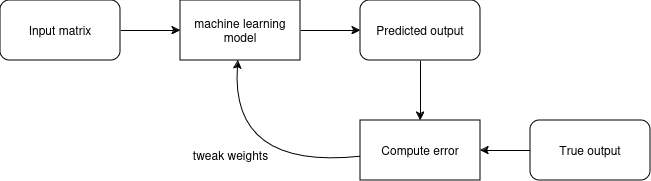
\includegraphics[width=\linewidth]{images/supervised_learning_diagram.drawio.png}
    \caption{The supervised learning method.}
    \label{fig:supervised_learning}
\end{figure}



\subsubsection{Input DAGs}
~

In machine learning, the input that we give to the model
needs to be in a matrix representation so that the model can 
then process it. Therefore, every DAG task needs to have
a matrix representation that encompasses the information 
required to make decisions about its execution priority order.  
Each input DAG task will be represented using 
a matrix of numbers with each row being a node
and each column being a raw feature of a node.
The list of raw features is similar to what is proposed by \citet{Lee2021GlobalDagSchedDRL},
that is :
\begin{list}{}{}
    \item - the normalized wcet of the node, i.e., $C_i / L$ for node $i$ with $L$ being the total workload ;
    \item - the number of incoming neighbours ;
    \item - the number of outgoing neighbours ;
    \item - a boolean value of whether the node is the source or sink node ;
    \item - a boolean value of whether the node is part of the critical path of the DAG.
\end{list}

The wcet is widely used as a criteria for priority-list scheduling algorithm (RM, EDF\cite{buttazzo2005RMvsEDF}, etc.)
but it needs to be normalized to have the context information of the whole graph.
The number of incoming and outgoing neighbours makes it possible 
to take into account the inner structure of the graph to compute the execution order.
The source and sink nodes are particular nodes in that their priority
is not important because they will respectively execute first and last due to their dependency constraints.
Finally, the critical path plays a huge role in state-of-the-art heuristics\cite{He2019DagIntra}\cite{zhao2020DAGsched},
with nodes in the critical path often having higher priorities than those
that aren't.
An example of such a DAG task representation is shown in Figure \ref{fig:dag_task_matrix_example}.

\begin{figure}
    \centering
    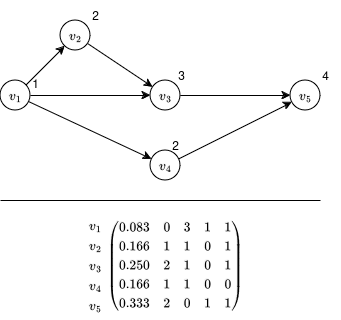
\includegraphics[width=\linewidth]{images/dag_matrix_example.drawio.png}
    \caption{Example dag task with 5 nodes a total workload of 12
    and the matrix representation of each node with the column respectively being the above list of features.}
    \label{fig:dag_task_matrix_example}
\end{figure}

\subsubsection{Output labels}
~
\label{sec:output_labels}

In order for the supervised model to learn, it needs to 
compare its predicted output against a known-to-be-true output, also 
called an output label. In this case,
the output label is supposed to be an optimal priority-list

Therefore, an Integer Linear Programming (ILP) solver will be used to compute
the optimal (minimum makespan) schedule for each DAG task and then
ordering the nodes according to their release time in the ILP schedule.

The output of the model will be a matrix of probabilities,
with each row being the index of a node and each column being the index of the priority.
There are as many priorities as there are nodes and 
the priority list of each DAG is then retrieved using the column
index of the maximum probability as the assigned probability, for each row.
Matrix output example for the DAG task shown in Figure \ref{fig:dag_task_matrix_example}
is shown in Figure \ref{fig:dag_output_matrix_example}.

\begin{figure}
    \centering
    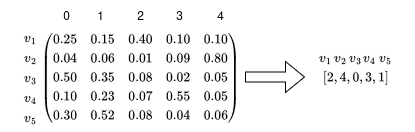
\includegraphics[width=\linewidth]{images/output_matrix_example.drawio.png}
    \caption{Example of an matrix output from the model, the predicted list of priorities (on the right)
    is retrieved from the probabilities.}
    \label{fig:dag_output_matrix_example}
\end{figure}

The ILP output matrix to compare the predicted output to is of the same shape
as the predicted output matrix with the probabilities being 1 on the optimal priority for each row 
, and 0 otherwise. For instance, if the optimal priority list for a DAG task of 3 nodes 
is [$\tau_1$: 0, $\tau_2$: 2, $\tau_3$: 1],
then the true label is the matrix :
$$
\begin{pmatrix}
    1 & 0 & 0\\
    0 & 0 & 1\\
    0 & 1 & 0
\end{pmatrix}
$$
With each row representing $\tau_1$, $\tau_2$ and $\tau_3$ respectively,
and the column represent the priorities 0, 1 and 2 respectively.
\subsubsection{Loss function}
~
\label{sec:loss_design}

The problem is being treated as a classification problem,
hence the binary cross-entropy loss function will be used.
This function is defined as follows :
\begin{equation}
    loss(x, y) = \sum_{i=1}^{n} -y_i\log(x_i)
\end{equation}
    
where $x$ is the flattened matrix representing the predicted output,
$y$ is the flattened matrix representing the true output (ILP output),
and $n$ is the number of element in $x$ and $y$.


\subsection{Model design}
~
\label{sec:model_design}

The model's architecture is very similar to the proposed encoder in \citet{Lee2021GlobalDagSchedDRL},
that is, the model is comprised of three modules.
Two feed forward networks and one attention-based graph convolutional network (see Figure \ref{fig:model_diagram}).

\begin{figure}
    \centering
    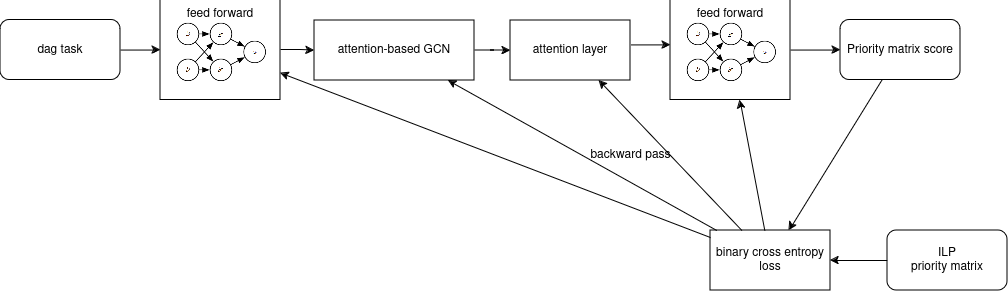
\includegraphics[width=\linewidth]{images/designed_model.png}
    \caption{The architecture diagram of the proposed supervised machine learning model.}
    \label{fig:model_diagram}
\end{figure}

\subsubsection{Feed forward networks}
~

The two feed forward networks have 3 layers with each 
layer $n$ producing the following output,
where $W_n \in \mathbb{R}^{5\times5}$ is the matrix of trainable weights
at layer $n$, $b_n \in \mathbb{R}^5$ is the bias and $X_n$ is either a node's vector representation
or the output of the previous layer, and $ReLU(x) = max(0, x)$:
\begin{equation}
    o_{n} = ReLU(W_{n}X_{n} + b_n),\, n \in \{1,2,3\}
\end{equation}
There is an exception for the second feed forward network where the last 
layer's output is computed using the following equation:
\begin{equation}
    o_{3} = \tanh(W_{3}X_{3} + b_3)
\end{equation}
where $W_3 \in \mathbb{R}^{nbPriorities \times 5}$,
$b_3 \in \mathbb{R}^{nbPriorities}$ and $\tanh$ is the 
hyperbolic tangent activation function.
Also, $nbPriorities$ corresponds to the number of different priorities
that can be assigned to each node.


\subsubsection{Graph Convolutional Network}
~

For each gcn layer, the input vector $X_k$ 
goes through an aggregation phase where,
given the set of incoming neighbours of node $v_i$, $\mathcal{N}_{in}(v_i)$, which includes
$v_i$, and the set of outgoing neighbours $\mathcal{N}_{out}(v_i)$, which also includes $v_i$,
the next vector representation $X_{k+1}$ is calculated by the following equation:

\begin{equation}
GCN(X) = AttentionModule(X, \mathcal{N}_{in}(v_i), \mathcal{N}_{out}(v_i))
\end{equation}

where $AttentionModule$ is defined by the Equations \ref{eq:attention_module}--\ref{eq:elu}:

\begin{multline}
    AttentionModule(X, \mathcal{N}_{in}(v_i), \mathcal{N}_{out}(v_i)) = \\
    ELU\left( W \left( Att(X, \mathcal{N}_{in}(v_i)) \oplus Att(X, \mathcal{N}_{out}(v_i)) \right) + b \right)
    \label{eq:attention_module}
\end{multline}

\begin{equation}
Att(X, \mathcal{N}(v_i)) = W\sum_{j \in \mathcal{N}(v_i)} \alpha_{ij} X_j
\label{eq:attention_submodule}
\end{equation}
Where 
\begin{equation}
    \alpha_{ij} = \frac{\exp \left ({ a ^{T} W X_{i} + b ^{T} W X_{j} }\right )}
    {{\sum _{k \in \mathcal {N}(v_{i})}} \exp \left ({ a ^{T} W X_{i} + b ^{T} W X_{k} }\right )}
\end{equation}

are the attention coefficients
which evaluates how important is $v_j$ to $v_i$'s vector 
representation, similar to what is done in \citet{Lee2021GlobalDagSchedDRL}.

Every $W$, $a$, and $b$ are different matrices of trainable parameters,
and $\text{ELU}$ is the exponential linear unit activation function (Equation \ref{eq:elu}).

\begin{figure}
    \centering
    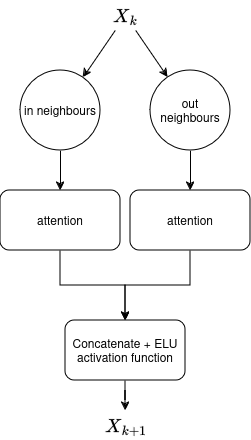
\includegraphics[width=0.5\linewidth]{images/gcn_update_aggregate_diagram.png}
    \caption{Diagram of the graph convolution network layer. $X_k$ is the transformed node vector representation
    and ELU is the exponential linear unit function (see Equation \ref{eq:elu}).}
    \label{fig:update_aggregate_diagram}
\end{figure}

\begin{equation}
\text{ELU}(x) = 
\begin{cases}
x, & \text{if } x > 0 \\
\exp(x) - 1, & \text{if } x \leq 0
\end{cases}
\label{eq:elu}
\end{equation}


The idea behind using attention is to make the model 
take into account the inner structure of the graph by 
looking at the importance of each node
compared to its neighbour nodes.
The GCN layer can be repeated several times 
to improve the model's capacity to better
capture the complexity of the graph structure.
Unfortunately, when testing with 3 GCN layers,
we ran into an oversmoothing problem\cite{chen2020oversmoothing}, which lead us 
to restrict the number of GCN layers to just one layer.

\subsection{Computing the labels}
~

\subsubsection{Computing the optimal schedule}

\citet{yip2023letsynchronise} proposed an ILP-based
scheduling solver for event-chains of time-triggered tasks
using the Logical Execution Time paradigm\cite{kirsch2012logical}.
Their work aimed at minimizing the sum of dependency delays 
between the job instances of each task and they have recently added
support for multicore architectures\footnote{https://github.com/mkuo005/LET-LP-Scheduler}.

Although their minimizing problem is slightly different from ours, 
we can convert our minimizing problem and then use their LET solver by converting each DAG task 
to an event-chain of LET task.
To do this, each node needs to be converted to an LET task which 
implies adding an initial offset, activation offset, LET interval duration and a period
to every node.
Hence, for each node, the initial offset and activation offset will
be set to 0 and the LET interval duration will be set to the node's wcet.
For the period, every node in a DAG will have the same period which will
be equal to the total workload squared.
The wcet of a node will be the wcet of its LET task version.
Lastly, each path in the DAG will represent an even-chain of tasks.

Unfortunately, minimzing the sum of dependency delays (i.e., Equation 6 in \citet{yip2023letsynchronise}) is not equivalent
to minimizing the makespan of a DAG (see Figure \ref{fig:counter_example_minsumdep})
but we can change the objective function to the end execution time
of the sink node, i.e., the node which doesn't have any successors,
which is the definition of the makespan.
This effectively makes the solver minimize the makespan of DAG task
which is precisely the problem at stakes.
The other modifications involve setting the configuration parameters $useOffset$,
$useHeterogeneousCores$ and $restrictTaskInstancesToSameCore$ to
$False$\footnote{See the github repository for more details \url{https://github.com/FelicienFG/research-project-AUT/}.}.

\begin{figure}
    \centering
    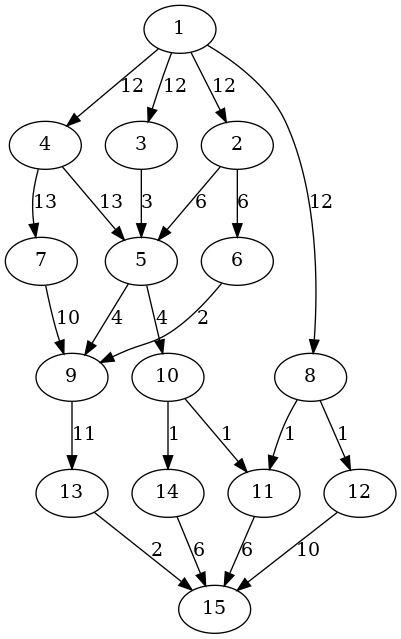
\includegraphics[width=0.5\linewidth]{images/Tau_108.png}
    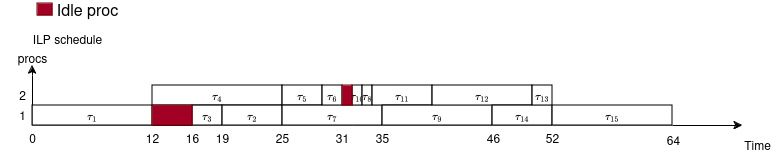
\includegraphics[width=\linewidth, height=70px]{images/schedule_ilp_fail_correct.png}
    \par Schedule a)
    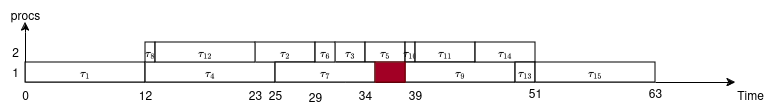
\includegraphics[width=\linewidth, height=55px]{images/schedule_example_ilpfail_better.png}
    \par Schedule b)
    \caption{Example of a DAG task (top image) where the schedule that the ILP solver outputs (the schedule a))
    produces a longer makespan (64) but smaller sum of dependencies delays (400) than 
    the schedule b) with a makespan of 63 and a sum of dependencies delays of 427.}
    \label{fig:counter_example_minsumdep}
\end{figure}

\subsubsection{Computing the optimal priority-list}
~

Once the optimal schedule (i.e., the schedule yielding the minimum makespan)
is computed,
the optimal priority-list can be obtained from the schedule 
by looking at the start times of each node and increasing the priority 
according to the node's start time.
The sooner the start time, the higher the priority.

For instance, for the non-optimal schedule shown in Figure \ref{fig:counter_example_minsumdep} (schedule a)),
the corresponding priority-list would be 0 for node $\tau_1$, 1 for node $\tau_4$,
etc, i.e., [$\tau_1$: 0, $\tau_2$: 3, $\tau_3$: 2, $\tau_4$: 1, $\tau_5$: 4, $\tau_6$: 6, $\tau_7$: 5, $\tau_8$: 8,
 $\tau_9$: 10, $\tau_10$: 7, $\tau_11$: 9, $\tau_12$: 11, $\tau_13$: 13, $\tau_14$: 12, $\tau_15$: 14].
This priority list is then converted to a matrix by the process described
at the end of Section \ref{sec:output_labels}.

\subsection{Makespan calculation}
~

The main performance metric that will be used in the evaluation
is the makespan, i.e., the end execution time of the sink node of a DAG.
The exact computation of the makespan is done by simulating a 
simple non-preemptive global fixed-priority scheduler, for which the algorithm
is described in the Figure \ref{fig:algo_makespan}.
The basic idea is to have a ready queue that contains the nodes
that have their precedence constraints met
and the nodes still waiting to have their dependencies met 
are in the waiting list. Each loop iteration, the waiting list and ready queue
are updated and the first idle processor gets the node at the top of 
the ready priority queue (see Figure \ref{fig:algo_makespan} and \ref{fig:algo_makespan_details}).

\begin{figure}
    \centering
    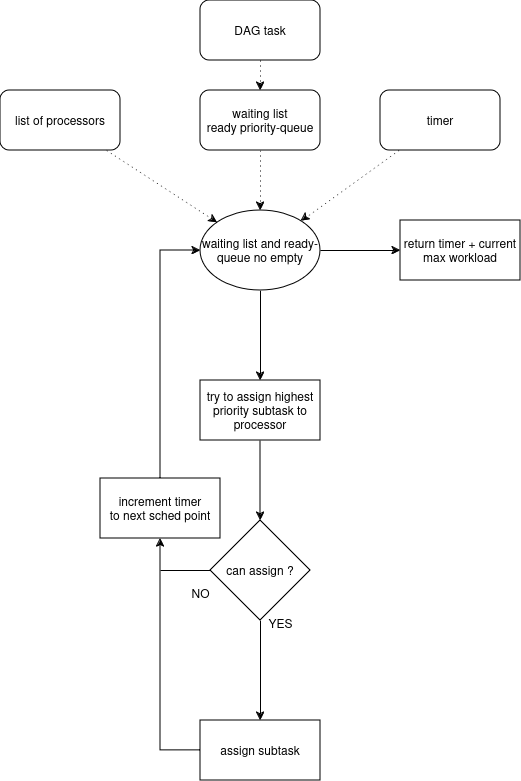
\includegraphics[width=\linewidth]{images/makespan_computation_algorithm_global.png}
    \caption{Top view of the makespan computation algorithm.}
    \label{fig:algo_makespan}
\end{figure}

\begin{figure}
    \centering
    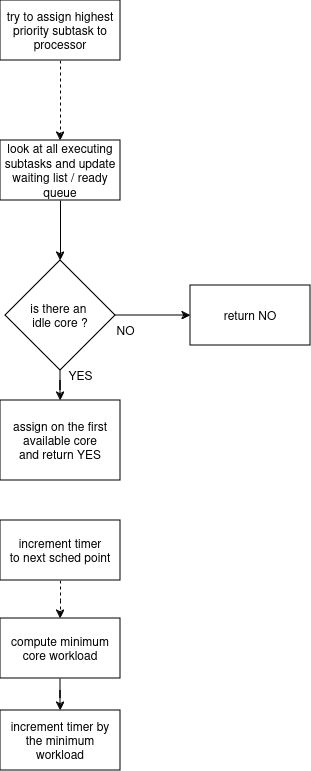
\includegraphics[width=0.8\linewidth]{images/makespan_computation_algorithm_assign.png}
    \caption{Algorithms for assigning the highest priority node (or subtask) to a processor (top)
    and for incrementing the timer to the next scheduling point (bottom).}
    \label{fig:algo_makespan_details}
\end{figure}

The implementation will be done in C++ with bindings to python to make
the makespan computation faster.

% config for 20,30 nodes : 
%  "dag_config": {
%    "parallelism": 8,
%    "layer_num_min": 5,
%    "layer_num_max": 8,
% config for 10 nodes :
%"dag_config": {
%    "parallelism": 8,
%    "layer_num_min": 3,
%    "layer_num_max": 8,
% config for 40 nodes :
%"dag_config": {
%    "parallelism": 8,
%    "layer_num_min": 7,
%    "layer_num_max": 10,
% config for 50 nodes :
%"dag_config": {
%    "parallelism": 8,
%    "layer_num_min": 10,
%    "layer_num_max": 15,
%config for varying number of parallelism (n=30nodes)
%"dag_config": {
%    "parallelism": [4-6, 7],
%    "layer_num_min": 8, (5 for p = 7)
%    "layer_num_max": 13, (10 for p = 7)
\section{Evaluation}
~

\subsection{Environment setting}
~

The evaluation of the model is focused on two metrics : the makespan and the computing time once trained.
For the implementation of the model, python 3.10.12 with the PyTorch 2.4.1 library is used and runs on a google collab runtime
with 90 TPU cores.
The stochastic gradient descent is used for training with a learning rate of $0.001$ and a batch size of 250.

During the initial evaluation, an over-smoothing problem\cite{chen2020oversmoothing} occured which lead to 
the model smoothing out the priorities and assigning the same priority to all the nodes.
To try to solve this, reducing the number of GCN layers to 1 was done,
which unfortunately didn't fix the problem, leading to the addition
of a regularization term to the loss function.
The idea is to tackle the over-smoothing probblem by forcing the model
to differentiate between the nodes' representation.
Hence, the regularization term is the squared inverse of the average euclidian distance 
between each of the nodes' latent representation, i.e., 
\begin{equation}
    \text{regTerm}(X) = \frac{1}{\sum_{i}\sum_{j > i} \Vert X_i - X_j\Vert_{2} }
\end{equation}
    
and the loss function then becomes
\begin{equation}
    loss(X, y) = \sum_{i} -y_i\log(x_i) + \text{regTerm}(X)
\end{equation}
with $x_i$ being the elements in $x$, the flattened matrix representation of $X$
and $y$ the true output (see Section \ref{sec:loss_design}).

Although those modifications didn't seem to improve on the initial results,
the evaluation of the model has been done with these modifications
to establish why the over-smoothing problem was happening(see Section \ref{sec:discussion}).

\subsection{Dataset generation}
~

To generate the DAG tasks, the generator from \citet{zhao2020DAGsched} is used, which is also used by 
\citet{Lee2021GlobalDagSchedDRL} and \cite{Zhao2022DAGsched}, to generate
random DAGs.
Apart from it being used by state-of-the-Art papers, which my results will be compared to,
and providing a qualitative and diverse dataset,
this generator has great modularity and the open-source git repository\footnote{https://github.com/automaticdai/dag-gen-rnd} 
makes it easy-to-use.
The random DAGs are generated using the following process :
The generator starts at a source node and expands outward, 
creating nodes in successive layers. The total number of layers, 
or maximum depth, is randomly determined to be between two values $a$ and $b$.
For each layer, the number of nodes generated is chosen uniformly, 
ranging from 2 up to the parallelism parameter, $p$ which in this case, 
is fixed at $p=8$. Nodes that do 
not already have connections can randomly connect to other nodes in 
the previous layer with a probability of $p_c=0.5$. After all layers 
are generated, any terminal nodes are linked to a final sink node. 
Both the source and sink nodes are used to structure the graph and 
have a fixed execution time of one unit each. Lastly, 
execution times are assigned randomly to all nodes while ensuring 
that the total workload sums up to $W = 1000$\cite{zhao2020DAGsched},
that is, the fully sequential execution time of each DAG task is set to 1000 time units (i.e., the sum of each node's wcet).

To generate DAGs with a fixed number of nodes $n$, 
the generator is first used to generate 50000 DAG tasks
with different values for $a$ and $b$ depdending on what 
the value of $n$ is. Then, the generated DAGs with 
the specified number of nodes are retrieved from the dataset.
Specifically, Table \ref{tab:layer_num_minmax} 
shows the different $a$ and $b$ values according to $n$.

\begin{table}
    \centering
    \begin{tabular}{|c|c|c|}    
        \hline
        \textbf{n} & \textbf{a} & \textbf{b} \\
        \hline
        10 & 3 & 8 \\
        \hline
        \{20, 30\} & 5 & 8 \\
        \hline
        40 & 7 & 10 \\
        \hline
        50 & 10 & 15 \\
        \hline
    \end{tabular}
    \caption{dag generator $a$, minimum number of layers, and $b$, maximum
    number of layers, parameter values for generating 
    random DAGs according to number of fixed nodes per graph we need to retrieve afterwards.}
    \label{tab:layer_num_minmax}
\end{table}

Using those values, 1400 DAG tasks were retrieved and used for 
evaluation, for each value of $n$.
1000 of them were used for training the model, 400 for testing
and 100 of them were used to measure the computing time 
for both the ILP and the supervised ML methods.


\subsection{Computing time results}
~

The computing time for the ILP method is shown 
in Figure \ref{fig:ilp_compute_time}.
The ILP solver was timed out whenever the computing time exceeded 1 hour
and it did time out when considering systems of 2 and 4 cores, when the number of nodes
exceeded 20 nodes (i.e., 30, 40 and 50 nodes) per DAG task.
Hence, in the next sections, only 6 and 8 cores will be considered,
with the number of nodes not exceeding 30 nodes, to have enough
ILP solved DAGs for training the model. 

\begin{figure}
    \centering
    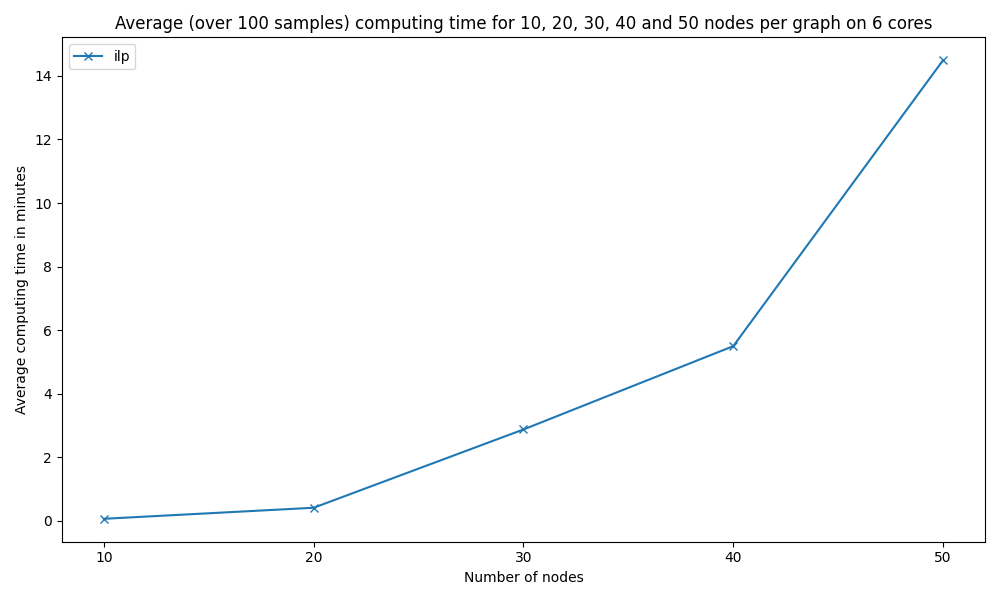
\includegraphics[width=\linewidth]{images/result_computing_time_ilp_m6.png}
    \caption{Average computing time for computing the optimal schedule
    of a single DAG task using the ILP method, in minutes, according to 
    the number of nodes in the DAG, on a system with 6 cores.}
    \label{fig:ilp_compute_time}
\end{figure}

As you can see from Figure \ref{fig:ilp_compute_time}, the more nodes there are on the system, 
the more time it takes for the ILP solver to compute the optimal schedule,
and it does so in, what it seems to be, an exponential growth.
Figure \ref{fig:ilp_compute_time} thus shows the non-scalability
of the ILP method, with the number of nodes per DAG increasing.

\begin{figure}
    \centering
    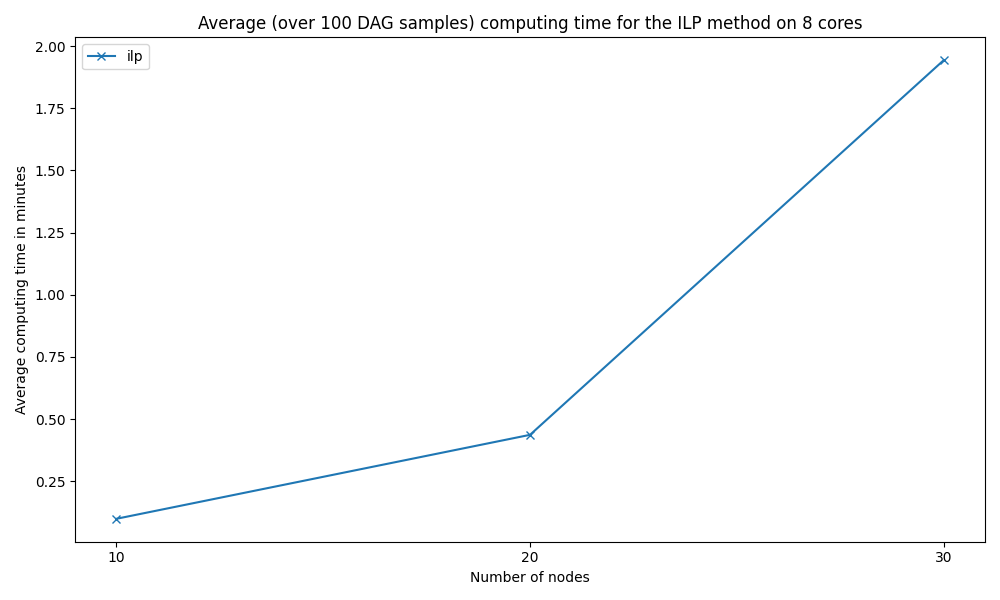
\includegraphics[width=\linewidth]{images/result_computing_time_ilp_m8.png}
    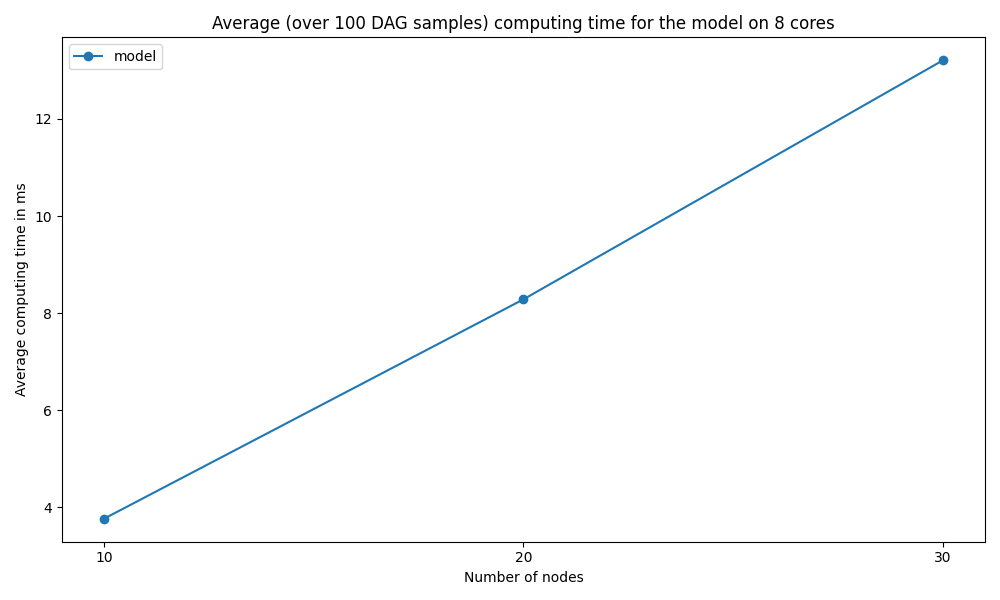
\includegraphics[width=\linewidth]{images/result_computing_time_model_m8.png}
    \caption{Average computing time for computing the optimal schedule
    of a single DAG task using the ILP method (top), in minutes,
    and using the ML model (bottom) according to 
    the number of nodes in the DAG, on a system with 8 cores.}
    \label{fig:compute_time_ilp_model}
\end{figure}

When comparing to the ML model's computing time (Figure \ref{fig:compute_time_ilp_model}),
you can see how, unlike ILP, the model seems to be a lot more scalable
than ILP, as shown by the linearity of the computing time curve (bottom graph of Figure \ref{fig:compute_time_ilp_model}).
The linearity is of course not a true linearity as the theoretical complexity,
in terms of operations on the nodes' vector representation,
of the model can be calculated to be $O(n^2)$ according to Section \ref{sec:model_design},
but the curve is linear because of how short the X axis is,
the polynomial curve is zoomed in which explains why the curve seems linear.

This difference in scalability is expected as the problem is NP-hard,
which means that the ILP solution, calculating optimal solutions,
has to be at least of exponential complexity, hence the non-scalability of the ILP method.
The model's scalability is also expected as the theoritacl complexity
is polynomial.


\subsection{Performance comparison}
~

Two performance metrics will be used for the model.
The makespan which will be compared to the ILP solution, the heuristic
from \citet{zhao2020DAGsched} and a random method where each priority is assigned at random,
and the accuracy / loss of the model.

\begin{figure}
    \centering
    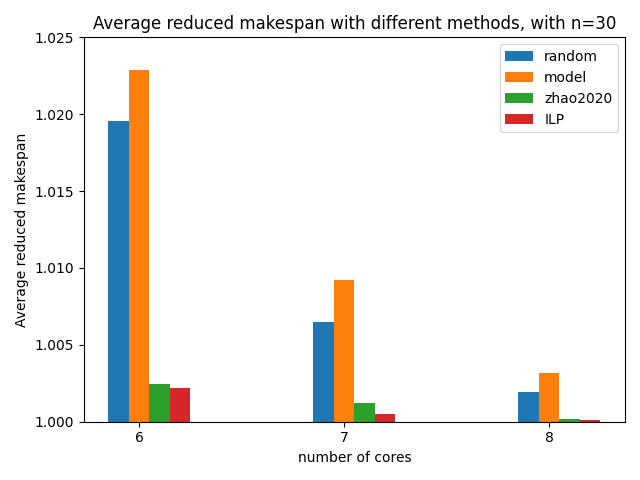
\includegraphics[width=\linewidth]{images/avg_makespan_n30.png}
    \caption{Average reduced makespan (makespan divided by the critical path length) on the test set (400 DAGs) using the four different methods
    on 6, 7 and 8 cores with 30 nodes per DAG,
    with 'random' being the method of randomly assigning priorities to nodes of a DAG.}
    \label{fig:avg_makespan_comparison_trained}
\end{figure}

Figure \ref{fig:avg_makespan_comparison_trained} shows the average
reduced makespan, which is the makespan divided by the length of the critical path,
computed with each method on 400 DAGs from the test set.
Therefore, the closer to 1 it is, the better it performs.

Not only does the model perform worse than the heuristic from \citet{zhao2020DAGsched},
the model performs generally worse than the random method.
Also, the heuristic is very close to matching the ILP method,
performing even greater than expected.

When not-trained (Figure \ref{fig:avg_makespan_comparison_untrained}), the model performs 
about the same or worse than randomly.
This is because although the weights are initialized randomly,
the similarity between the nodes' vector representation
makes the model, even when untrained, 
compute the same priority for different nodes, which 
is exacerbated with training, leading to the over-smoothing
issue (see Table \ref{tab:similarity_percentages}).


\begin{figure}
    \centering
    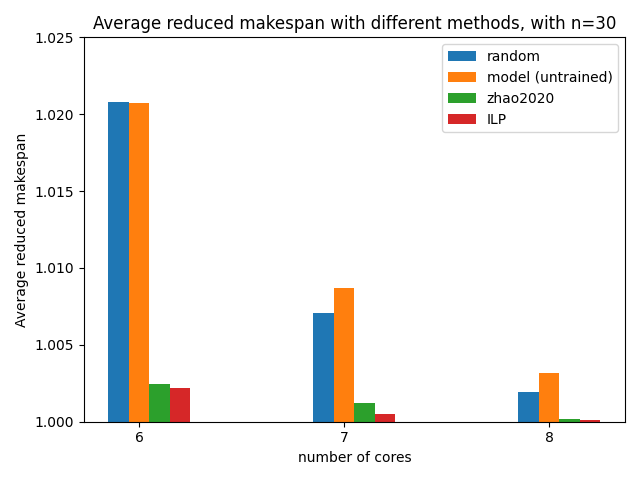
\includegraphics[width=\linewidth]{images/avg_makespan_n30_untrained.png}
    \caption{Average reduced makespan (makespan divided by the critical path length) on the test set (400 DAGs) using the four different methods
    on 6, 7 and 8 cores with 30 nodes per DAG,
    with 'random' being the method of randomly assigning priorities to nodes of a DAG,
    and the model not being trained.}
    \label{fig:avg_makespan_comparison_untrained}
\end{figure}


In terms of accuracy and loss, the results are shown in Figure \ref{fig:accu_loss_model}.
The accuracy is, in this case, how well the resulting priority list 
from the model matches the ILP priority list.
Unfortunately, the accuracy is stagnant at less than 10\%
and doesn't get better when increasing the number of epochs to train on. 
Also, the accuracy doesn't change between the training and testing phase
which further confirms that the model doesn't learn at all.

\begin{figure}
    \centering
    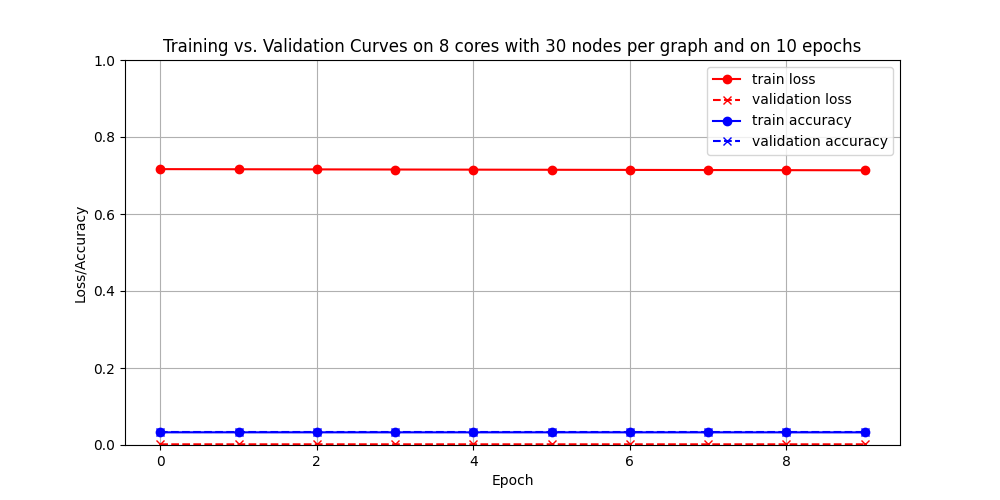
\includegraphics[width=\linewidth]{images/train_val_curves_m8n30epo10.png}
    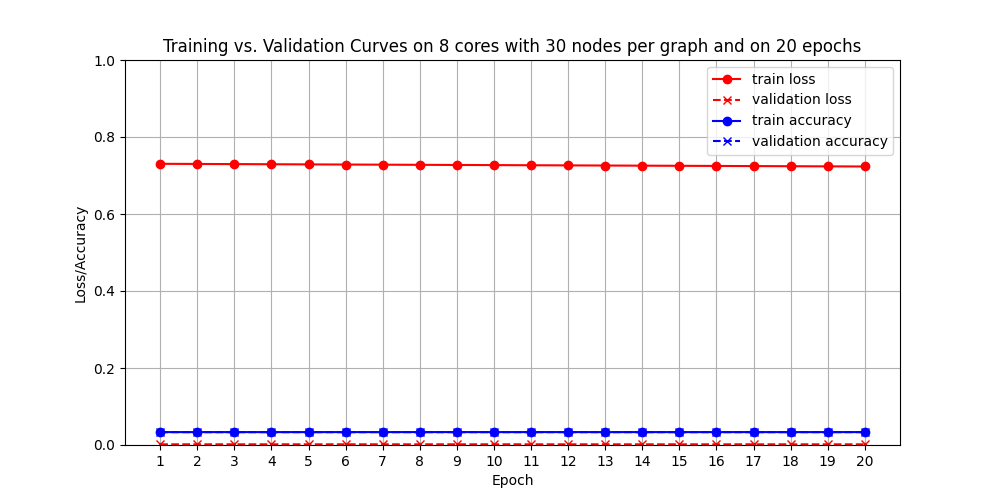
\includegraphics[width=\linewidth]{images/train_val_curves_m8n30epo20.png}
    \caption{Accuracy (in blue) and loss (in red) values for training (circles) and testing (crosses),
    accross the epochs. The top graph shows results for 10 epochs
    and the bottom one for 20 epochs. The results are shown on 8 cores with 30 nodes per DAGs,
    with a training batch size of 250 and a learning rate of $0.001$.}
    \label{fig:accu_loss_model}
\end{figure}

Furthermore,
when looking at the output of the model (Table \ref{tab:similarity_percentages}),
we can see that in most cases,
the priority lists predicted by the model are, on average, more than 90\% 
made out of the same value, i.e., for 10 nodes : [1, 1, 1, 1, 1, 1, 1, 1, 2, 1] for instance.
This shows that the over-smoothing of the DAGs is still an issue for the model and explains
the low accuracy.

\begin{table}
    \begin{tabular}{|c|c|c|c|}
        \hline
        \textbf{number of nodes per DAG/number of cores} & \textbf{6} & \textbf{7} & \textbf{8}\\
        \hline
        \textbf{10} & 94\% & 99\% & 94\%\\
        \hline
        \textbf{20} & 91\% & 60\% & 90\%\\
        \hline
        \textbf{30} & 100\% & 99\% & 98\%\\
        \hline
    \end{tabular}
    \caption{Average percentage of the number of priority slots that have the same value
    in a priority-list outputed by the model.}
    \label{tab:similarity_percentages}
\end{table}


Although the accuracy results shown here are only 
in the case of 8 cores and 30 nodes per DAG,
the other cases, i.e., for 6, 7 cores and with 10,20 and 30 nodes per DAG,
display very similar results and lead to the same conclusions as those
shown here.

\subsection{Discussions}
~
\label{sec:discussion}

There are several reasons why a machine learning model
sub-performs.
The issue can be because of an overfitting problem,
meaning that the model is too complex and learns the noise / bias
that comes with the dataset.
It can also be the opposite, under-fitting, 
which is due to a model that is too simple for the task at stake,
lacking the architecture to capture the complex information and 
relationships
in the data.
It can be because of the nature of the dataset that is too biased
or too noisy which makes it impossible for the model to learn from it.
Finally, it can be because the model didn't train on enough data 
or on enough epochs, which would mean that the model didn't have
the time to converge and need more data samples to do so.

Let's tackle these different problems and see why 
the problem is the fact that supervised-learning isn't fit for this kind of problem,
that is the single DAG task scheduling problem.


\subsubsection{Biased data and amount of data}
~

Data is always bias and the amount of dataset bias\cite{torralba2011biasdataset}
can have a huge impact on the performance of a model.
Although the number of training samples (1000) is not a lot 
compared to what \citet{Lee2021GlobalDagSchedDRL} have generated (8000),
the dataset generation procedure is the same as the one 
in both \citet{zhao2020DAGsched} and \citet{Lee2021GlobalDagSchedDRL}.
The latter specifically, got more than promising results with their machine learning model,
outperforming the heuristic in \citet{zhao2020DAGsched} by up to 3\% in terms of makespan,
 when using the same data generation procedure as here.
Furthermore, the loss is extremely stable and doesn't go down
during training, even when training on 20 epochs (Figure \ref{fig:accu_loss_model}).
This means that even if there is bias in the data, the fact that others have used
the same data generation procedure and got great results shows that the
dataset bias cannot explain the low performance of the model.
Also, the fact that the model doesn't seem to learn at all with 
its loss being stagnant accross the epochs, removes the 
idea of the model performing badly because there is not enough data to learn on.


\subsubsection{Over-fitting or under-fitting}
~

The reason why the model is performing this badly is probably
not over-fitting.
This is because over-fitting is characterized
by the model learning the noise in the training set and performing\cite{jabbar2015overfitting_underfitting}.
Hence, if it were the case, there would be a noticable gap
between the training and validation accuracy in Figure \ref{fig:accu_loss_model},
which there isn't.
Also, the over-smoothing problem, which is causing the model to sub-perform,
 doesn't come from the noise
in the data but rather from the architecture of the model itself\cite{chen2020oversmoothing}.
Hence the problem might rather be that the model is under-fit for this problem.

Indeed, as mentioned before, what the model is learning is 
to assign the same priority at every node, which also means
that it doesn't learn to approximate the output given by the ILP priority-lists,
as shown by the accuracy and loss values not notably decreasing during
training (Figure \ref{fig:accu_loss_model}).
The issue here is that the model resembles very closely the 
encoder in \citet{Lee2021GlobalDagSchedDRL} which didn't 
have the over-smoothing problem.
The attention-mechanism used is also close to what is done in \citet{Zhao2024GATDRLmodel}
which also didn't have an over-smoothing problem.

The fact that The over-smoothing is very strong (see Table \ref{tab:similarity_percentages})
and that the model is close to what has been done in the reinforcement learning models\cite{Lee2021GlobalDagSchedDRL}\cite{Zhao2024GATDRLmodel},
lead us to conclude that the problem might be the learning method, 
that is the supervised learning method.

\subsubsection{the supervised learning problem}
~

In supervised learning, the problem is either going to be a
regression problem, when dealing with real numbers as the target variable
such as predicting the price of a product or the rate of infection in an epidemic, etc.
Or the problem is going to be interpreted as a classification problem.
In our case, the numbers are discrete and the set of priorities is finite
which is why the problem was treated as a classification problem.
However, usually, for supervised learning, the predicted output 
aim at mathing a ground truth, known beforehand, that is unique.
Although the ILP method permitted us to have a priority list that
effectively yields the minimum makespan,
that priority list is not unique.

Indeed, not only is the minimum makespan schedule not necessarily unique
(see Figure \ref{fig:not_unique_schedules}),
which means that the optimal priority-list is not unique
(in Figure \ref{fig:not_unique_schedules}, schedule a) gives 
[0, 1, 2, 3, 4, 5] but schedule b) gives [0, 1, 2, 4, 3, 5]).
But even if the schedule might be unique, when the start time
of nodes are the same, multiple priorities
can be assigned to those nodes.
For instance, in schedule a) of Figure \ref{fig:not_unique_schedules},
the  two priority-lists [0, 1, 2, 3, 4, 5] and [0, 2, 1, 3, 4, 5]
are valid for minimizing the makespan of the DAG.

\begin{figure}
    \centering
    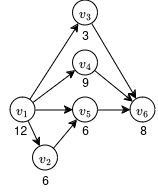
\includegraphics[width=0.5\linewidth]{images/dag_same_makespan_diff_scheds.png}
    \par a)
    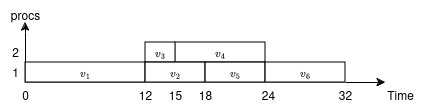
\includegraphics[width=\linewidth]{images/first_samemakespan_diff_sched.png}
    \par b)
    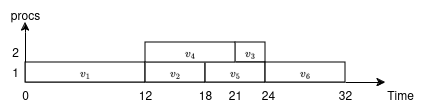
\includegraphics[width=\linewidth]{images/second_samemakespan_diff_sched.png}
    \par c)
    \caption{Example of DAG task (a) for which two schedules (b and c) leading to different
    priority lists are shown, both schedules giving the minimum makespan.}
    \label{fig:not_unique_schedules}    
\end{figure}


This complete lack of uniqueness in the true labels 
renders the ILP priority-lists almost useless
for the model to learn on, because those lists
don't show the difference between a node having 
a specific priority because it lengthen the makespan otherwise (e.g.,
priority of $v_8$ in the last two schedule scenarios in Figure \ref{fig:dag_schedule_example}),
and a node having a specific priority when it could have 
other potential priority values and it wouldn't change the makespan (e.g.,
the example in Figure \ref{fig:not_unique_schedules}).
Thus, the model can't learn to assign different priorities
to the nodes but rather to smooth out the priorities and give
the same one to most of the nodes of a DAG,
hence the over-smoothing problem.
Furthermore, the non-uniqueness in the nodes' vector representations
also contributes to the model struggling to learn.
Indeed, 
if two nodes have the same number of in and out neighbours,
are neither a sink nor a source node, their respective
vector representation will be very similar.
For instance, in the DAG shown in Figure \ref{fig:dag_same_representation_vector},
the vector representation of nodes $\tau_2$ and $\tau_3$ are the same,
i.e., $(0.067, 1, 1, 0, 0)$, and although those nodes having different priorities
doesn't impact the final makespan, they do have different priority values
with the ILP priority-list, which contributes to the over-smoothing problem. 
\begin{figure}
    \centering
    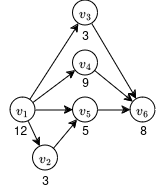
\includegraphics[width=0.5\linewidth]{images/dag_similarity_representation.png}
    \caption{Example of a DAG task where two different nodes have the
    exact same vector representation.}
    \label{fig:dag_same_representation_vector}
\end{figure}

One potential solution to explore might be to generate
, for each DAG, all the different schedules that lead to the minimum
makespan and from them, retrieve a single, unique priority list
not only containing the information about which nodes need to be
executed first, but also having the information of which nodes
have interchangeable execution ordering 
(e.g., the two nodes in the example above, Figure \ref{fig:dag_same_representation_vector}).
\\\\

The evaluation results show that the supervised learning model
doesn't learn correctly, leading to an over-smoothing and under-fitting problem
which makes the model perform very poorly (accuracy $<10$\%)
and having an even worse makespan performance than random priority assignment.
Analysis of the results showed how the model performance problem
is due to the learning method and supervised design being unfit for
the single DAG task fixed-priority scheduling problem.
Thus, relating to RQ3, although the reinforcement learning
method has shown great performance compared to ILP\cite{Zhao2024GATDRLmodel}
and state-of-the-Art heuristics\cite{Lee2021GlobalDagSchedDRL},
the supervised learning model presented here 
clearly cannot compare at all to either SOTA heuristics
or ILP, even though it is more scalable than ILP, 
mostly because of the supervised learning method being unsuited 
for DAG task fixed-priority scheduling.


\section{Experimental Results}
\label{sec:results}


\paraheading{Set up: what experiments/benchmarks were chosen?}


\paraheading{Execution of results: how were the experiments conducted}

\paraheading{Data: what was found to have happened?}


\paraheading{Synthesis: what does the data mean?}

\paraheading{Relevance: how does this work compare to others, and to what extent does it answer the RQs}

\paraheading{Limitations:}


\section{Conclusions and Future Works}









\section*{Acknowledgement}

\paraheading{For referencing in LaTeX, check out: \url{https://texblog.org/2014/04/22/using-google-scholar-to-download-bibtex-citations/}}


\bibliographystyle{IEEEtranN}
\bibliography{references}


\end{document}
